\subsection{Operation Model for oeSollicitateCrisisHandling}

\label{OM-oeSollicitateCrisisHandling}


The \msrcode{oeSollicitateCrisisHandling} operation has the following properties:

	\begin{operationmodel}
	\addheading{Operation}
	\adddoublerow{oeSollicitateCrisisHandling[proactive]}{A proactive message (message of a pro-active actor with no parameter triggered automatically if the pre protocol condition is true) used to avoid crisis to stay too long in an not handled status.}


	\addrowheading{Return type}
	\addsinglerow{ptBoolean}

	\addrowheading{Pre-Condition (protocol)}
	\addnumberedsinglerow{PreP}{the system is started}
	\addnumberedsinglerow{PreP}{ there exist some crisis that are in pending status and for which the duration between the current ctState clock information and the last reminder is greater than the crisis reminder period duration.}
		
	\addrowheading{Pre-Condition (functional)}
	\addnumberedsinglerow{PreF}{none}

	\addrowheading{Post-Condition (functional)}
	\addnumberedsinglerow{PostF}{if there exist coordinators and crisis who stood in a not handled status more than the maximum allowed time 
	then those crisis are randomly allocated to the existing coordinators.}
	\addnumberedsinglerow{PostF}{for all other crisis who stood too longly in a not handled status but not more than the maximum delay allowed 
	then a reminder message is sent to the administrator and all coordinator actors of the environment to sollicitate handling of those crisis.}

	\addrowheading{Post-Condition (protocol)}
	\addnumberedsinglerow{PostP}{the value of the last reminder known by the system at post state is the system's clock value.}
	\end{operationmodel}



	% ------------------------------------------
	% MCL Listing
	% ------------------------------------------
	\vspace{1cm}
	The listing~\ref{OM-actActivator-oeSollicitateCrisisHandling-MCL-LST} provides the \msrmessir (MCL-oriented) specification of the operation.
	
	\scriptsize
	\vspace{0.5cm}
	\begin{lstlisting}[style=MessirStyle,firstnumber=auto,captionpos=b,caption={\msrmessir (MCL-oriented) specification of the operation \emph{oeSollicitateCrisisHandling}.},label=OM-actActivator-oeSollicitateCrisisHandling-MCL-LST]

	/* Pre Protocol:*/ 
	preP{let TheSystem: ctState in
	  let AvpStarted: ptBoolean in
	  let ColctCrisisToHandle:
	        Bag(ctCrisis) in
	  
	  self.rnActor.rnSystem = TheSystem
	    
	/* PreP01 */
	  and TheSystem.vpStarted
	  
	/* PreP02 */
	  and TheSystem.rnctCrisis->select(handlingDelayPassed()) 
	      = ColctCrisisToHandle
	  and ColctCrisisToHandle->size().geq(1)}
	
	/* Pre Functional:*/
	preF{true}
	
	/* Post Functional:*/ 
	postF{let TheSystem: ctState in
	  let AMessageForCrisisHandlers: dtComment in
	  let ColctCrisisToAllocateIfPossible:Bag(ctCrisis) in
	  
	  self.rnActor.rnSystem = TheSystem
	/* PostF01 */
	  and TheSystem.rnctCrisis->select(maxHandlingDelayPassed())
	      = ColctCrisisToAllocateIfPossible
	  and  ColctCrisisToAllocateIfPossible->forAll(isAllocatedIfPossible())
	
	 /* PostF02 */
	  and TheSystem.rnctCrisis->select(handlingDelayPassed())
	  = ColctCrisisToHandle
	  
	  and ColctCrisisToHandle->msrColSubtract(ColctCrisisToAllocateIfPossible)
	      = ColctCrisisToRemind
	      
	  and if (ColctCrisisToRemind->size().geq(1))
	      then (AMessageForCrisisHandlers.value
	            ='There are alerts pending since more than the defined delay. Please REACT !'
	            and TheSystem.rnactAdministrator.
	                rnInterfaceIN^ieMessage(AMessageForCrisisHandlers)
	                and TheSystem.rnactCoordinator
	                    ->forAll(rnInterfaceIN^ieMessage(AMessageForCrisisHandlers))
	            )
	      else true
	      endif}
	
	/* Post Protocol:*/ 
	postP{ let TheSystem: ctState in
	  let TheClock: dtDateAndTime in
	  
	  self.rnActor.rnSystem = TheSystem
	  and TheSystem.clock = TheClock
	  and TheSystem@post.vpLastReminder = TheClock}
	
	\end{lstlisting}
	\normalsize 
	
	
	
	





Figure \ref{fig:lu.uni.lassy.excalibur.examples.icrash-OM-scopeView-operation-scope-outactActivator-oeSollicitateCrisisHandling}
shows concept model elements in the scope of the oeSollicitateCrisisHandling operation

\begin{figure}[htbp]
\begin{center}

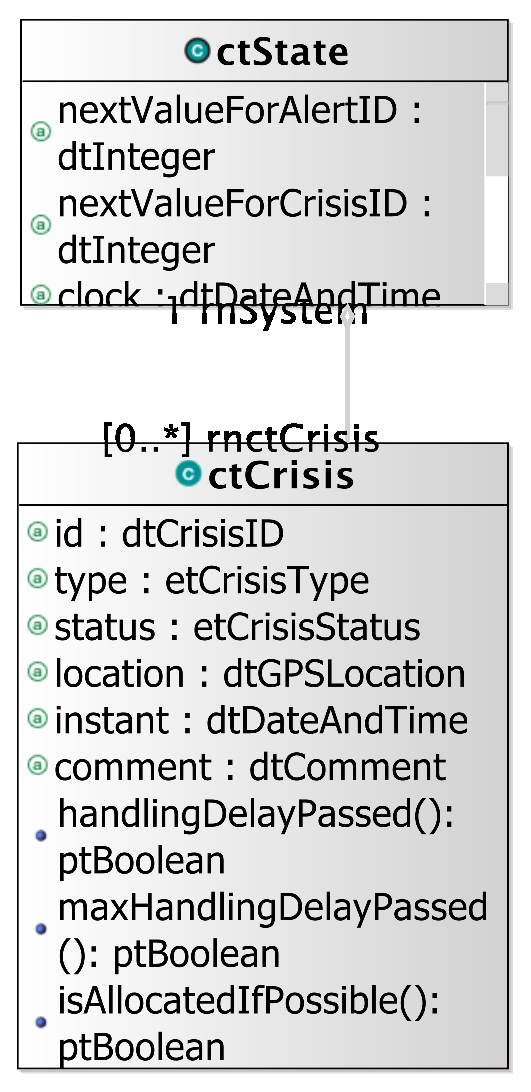
\includegraphics[
angle=0
,scale=0.75
]{./images-report-gen/operation-model/operation-scope-outactActivator-oeSollicitateCrisisHandling.eps}
\end{center}
\caption[lu.uni.lassy.excalibur.examples.icrash Operation Scope: operation-scope-outactActivator-oeSollicitateCrisisHandling]{oeSollicitateCrisisHandling operation scope
}
\label{fig:lu.uni.lassy.excalibur.examples.icrash-OM-scopeView-operation-scope-outactActivator-oeSollicitateCrisisHandling}
\end{figure}
\vspace{0.5cm}

